\chapter{Analyse}\label{ch:analyse}
Im Folgendem erfolgt eine Beschreibung der Beispielanwendung `Rechnungsschreibung`.
Die dafür benötigten Informationen stammen aus Gesprächen mit Mitarbeiter 1 aus der Abteilung, die für die Rechnungsschreibung zuständig ist.
Es wird vor allem der technische Aspekt beleuchtet.
Anschließend wird der aktuelle Bereitstellungsprozess für die Laufzeitumgebung, dem dazugehörigen Datenbanksystem und einer Messaging Lösung dargestellt.

\section{Rechnungsschreibung}
Für diese Arbeit wurde die Rechnungsschreibung als Beispielanwendung herangezogen, weil sie folgenden Anforderungen entspricht.
Es handelt sich zum einem um eine in sich abgeschlossene Anwendung, die nur zu Beginn des Prozesses von anderen Anwendungen abhängig ist.
Zum anderen benötigt die Rechnungsschreibung ein CICS als Laufzeitumgebung, eine Db2-Datenbank und MQ als Messaginglösung.
Somit kann ein umfangreicher Bereitstellungsmechanismus in dieser Arbeit untersucht werden.

\subsection{Beschreibung}\label{rechBesch}'DATEV Rechnungsschreibung' bezeichnet.\\
Bei dem Gesamtablauf handelt es sich um einen Batch\footnote{Stapelverarbeitung}-Ablauf auf dem Großrechner der DATEV e.G.
Nur die Preisermittlung ist als CICS-Anwendung implementiert.
Zunächst wird nach jeder kostenpflichtigen Leistungserbringung durch die dazugehörige Anwendung ein Berechnungssatz erzeugt.
Ein Berechnungssatz beinhaltet die Metainformationen der Berechnung unter anderem die Artikelnummer, Menge und den Ordnungsbegriff.
Preis und der Rechnungsempfänger werden zu einem späteren Zeitpunkt innerhalb der Rechnungsschreibung ermittelt.

\subsubsection{Einpflegung Berechnungssätze}
Für das Einpflegen der Berechnungssätze in den Rechnungsschreibungsablauf stehen den Anwendungen drei Möglichkeiten zur Verfügung.
DMVINF-MOdul
Webservice-Schnittstelle
CSV-Datei
\\
Bei der Ersten Möglichkeit handelt es sich um die Verwendung des DMVINF\footnote{DatevMakroVerarbeitungsinformation}-Moduls und der dazugehörigen Schnittstelle.
Das Modul ist in der Programmiersprache Assembler entwickelt.
Das Ergebnis des Moduls ist eine sequentielle Datei am Großrechner, vergleichbar mit einer .txt Datei unter Windows.
Diese Datei, auch Berechnungsdatei genannt, hat folgenden Aufbau.
Der erste Satz enthält Steuerinformationen, wie zum Beispiel Datum/Uhrzeit, Produkt usw.
Danach kommen die eigentlichen Berechnungssätze.
Schließlich folgt noch die Anzahl der Sätze und die Summe der einzelnen Artikel in einem Satz mit Kontrollinformationen.
Diese Kontrollinformationen werden im weiteren Verlauf mit den eingelesenen Werten abgeglichen, dadurch werden Datenverlust und unkontrollierte Eingriffsmöglichkeiten (Kommentar ... was ist damit gemeint? Sabotage? Fehler?)  von außen ausgeschlossen.
Aus dem Aufbau einer solchen Datei lässt sich schließen, dass verschiedene Schritte für die Erzeugung innerhalb der Anwendung notwendig sind.

Für die nachfolgenden Schritte stellt das DMVINF-Modul jeweils Schnittstellen zur Verfügung.
Zuerst wird beim sogenannten Open die Datei erstellt und der Steuersatz geschrieben.
Danach folgt das eigentliche Schreiben der Berechnungssätze, dabei dürfen nur bestimmte Felder (Ordnungsbegriffe, Länderschlüssel und Mengen) verändert werden.
Um unzulässige Veränderungen zu verhindert, haben diese einen Abbruch der Verarbeitung zur Folge.
Schließlich folgt noch der `Close` bei dem die Kontrollinformationen geschrieben werden.
Hinzuzufügen ist, dass die variablen Informationen einer Formalprüfung unterzogen werden.
So entstehen je nach fachlicher Logik und Laufhäufigkeit der Anwendung mehrere Berechnungsdateien. (Kommentar: ist diese Beschreibung relevant für die Anwendung???)

Eine weitere Möglichkeit, die Berechnungsinformationen in den Ablauf einzupflegen ist die Übergabe durch einen in der Programmiersprache Java realisierten WebService (Kommentar: Restful Service? SOAP?).
Hier werden die Berechnungsinformationen in XML-Format bereitgestellt.
Das Ergebnis der entsprechenden Plausibilitätsprüfungen, die in einem Onlineverfahren durchgeführt werden, wird direkt an die aufrufende Anwendung zurückgegeben.
Sind die Daten korrekt werden diese vorerst in einer Datenbank gespeichert.
Vor dem nächsten Schritt wird diese Datenbank ausgelesen und mit der ersten Möglichkeit in den Kernablauf eingespeist.

Bei der letzten Möglichkeit handelt es sich um die Übergabe mittels einer CSV-Datei.
Die Datei wird auf den Großrechner übertragen und dort mit dem DMVINF-Modul verarbeitet.
Dieses Verfahren wird kaum von produktiven Anwendungen sondern hauptsächlich für Test- oder Qualitätssicherungszwecke genutzt.

Mittels dieser drei Möglichkeiten werden insgesamt monatlich circa 30 Millionen Datensätze bereitgestellt und weiterverarbeitet.
Diese Datensätze stehen innerhalb der durch das DMVINF-Modul erzeugten Berechnungsdateien dem weiteren Verlauf als Input zur Verfügung.
Um sicherzustellen, dass all diese Dateien auch verarbeitet werden, wird bei Erstellung einer solchen (Kommentar was?) ein Eintrag in eine Kontrolldatei vorgenommen.
In dieser Kontrolldatei wird jedes Lesen und somit auch das Lesen im weiteren Verlauf gekennzeichnet.
Eine monatliche Überprüfung führt die zuständige Abteilung durch. (Kommentar: manuell???)

\subsubsection{Tägliche Bewertung}
Der nächste Schritt des Rechnungsschreibungsprozesses ist die sogenannte 'Tägliche Bewertung'.
Dieser Ablauf läuft einmal täglich von Montag bis Freitag und ist für die Preis- und Rechnungsempfängerermittlung zuständig.
Zur Realisierung wurden die Programmiersprachen Assembler und COBOL genutzt.
Am Ende dieses Ablaufes steht die ARUBA\footnote{Abrechnungs- und Umsatz-Basis}-Db2-Datenbank.
Dort werden die Berechnungsdaten der letzten 36 Monate aufbewahrt.
Dabei handelt es ich um insgesamt circa 3,8 Milliarden Datensätze von einer Gesamtgröße von circa 400 GB mit Indizes.
Diese Datensätze beinhalten alle Informationen für die endgültige Erzeugung der Rechnungen.

Der erste Schritt der Täglichen Bewertung ist das Zusammenführen der Berechnungsdateien aus dem vorherigen Schritt und aus den bereits vorhandenen Daten des laufenden Monats aus der ARUBA-Db2-Datenbank.
Zusätzlich werden während dieser Zusammenführung den Berechnungssätzen auf Basis der abgebenden Anwendung die entsprechenden Rechnungsstellungsrythmen (täglich oder monatlich) zugewiesen.
Anschließend wird mit Hilfe der Beraternummer die zugehörigen Betriebsstätte-, Rechnungsempfänger-, Hauptberater- und Mitglieds- bzw. Geschäftspartnernummer ermittelt.
Die Beraternummer ist als oberster Ordnungsbegriff in den Berechnungssätzen enthalten.
Außerdem wird die Debitorenkontonummer entweder durch die Mitglieds- oder durch die Geschäftspartnernummer zugeordnet.
Für die Preisermittlung werden die Datensätze nach Geschäftspartner gruppiert.
Im DATEV eG Umfeld ist ein Geschäftspartner entweder eine Kanzlei oder ein einzelner Mandant, dieser ist jedoch meist einer Kanzlei zugeordnet. (Kommentar: meist? gibt es Mandanten ohne Kanzlei???)

Dann werden die gruppierten Daten in eine CICS-Anwendung übertragen. Die Entscheidung, die Anwendung in CICS zu hosten hatte die zuständige Abteilung aus Performancegründen getroffen) 
Die Architektur  der CICS-Anwendung wird in \ref{rechArch} beschrieben.
Dort findet die Preisermittlung mit den dazugehörigen kundenindividuellen Abhängigkeiten, wie zum Beispiel Rabatten, statt.
Anschließend werden die Daten wieder zurück an den Batch-Ablauf übertragen.
Hier werden die Rechnungsnettobeträge geprüft, z.B. ob diese über einem bestimmten Rechnungslimitbetrag liegen.
Ist alles in Ordnung werden die Berechnungssätze als BUL\footnote{Berater unter Limit} gekennzeichnet und in die folgende Rechnungsperiode vorgetragen.
Schließlich wird noch die Umsatzsteuer ermittelt.
Abschließend werden die neu erzeugten Berechnungsdaten in die ARUBA-Db2-Datenbank eingepflegt und entsprechend gekennzeichnet.

\subsubsection{Rechnungsaufbereitung}
Als letzter Schritt folgt die Rechnungsaufbereitung.
Diese erfolgt am ersten Werktag im Monat.
Mit Hilfe der ARUBA-Db2-Datenbank wird ermittelt, welchen Kunden eine Rechnung zugestellt werden muss.
Außerdem wird dabei der Zustellungsweg, Post oder E-Mail, bestimmt.
Darauf folgt die Aufbereitung der Druckrohdaten und letztlich das Versenden der Rechnungen an die Berater.
Zusätzlich werden die Rechnungen noch im PDF-Format archiviert.

\subsection{Architektur der Preisermittlung}\label{rechArch}
In dieser Arbeit steht das automatisierte Provisionieren von Laufzeitumgebungen im Fokus.
In diesem Fall handelt es sich um die Laufzeitumgebung CICS mit den dazugehörigen Elementen.
Deshalb wird im Folgenden nur auf die Anforderungen der Rechnungsschreibung an das CICS-System eingegangen.

Das System muss an Lasttagen bis zu 180.000 Geschäftspartner verarbeiten können.
Um all diese an das CICS zu übertragen, stehen dem System mehrere IBM MQ Queues zur Verfügung.
Bevor die eigentliche Ermittlung der Preise stattfindet, werden zunächst die Listenpreise ermittelt.
Hierfür werden zwei Queues verwendet.
Eine startet eine Transaktion im CICS, die andere wartet auf deren Antwort.
In diesem Ablauf werden die benötigten Listenpreise aus einer Datenbank ausgelesen und in einen Hauptspeicherbereich der CICS Instanz gespeichert.
Dies ist auf Grund der Last auf dem System notwendig, da ein Hauptspeicherzugriff schneller als ein Datenbankzugriff ist.
MIt der  Umstellung auf diese Logik konnte die Fachabteilung eine Laufzeitverbesserung um circa XXXX Prozent erreichen.

Für die Bestimmung der Preise mit den Preisabhängigkeiten bestehen weitere Queues.
Darunter ist eine allgemeine Queue in der alle Aufträge, die für die Weiterverarbeitung zur Verfügung stehen, geschrieben werden.
Pro Geschäftspartner wird ein Auftrag angelegt.
In diesem Auftrag befinden sich die Namen vier weiterer Queues.
Eine dieser Queues beinhaltet alle Informationen, die für die Preisermittlung des dazugehörigen Geschäftspartners notwendig sind.
In den restlichen drei Queues sind die Ergebnisse der Preisermittlung gespeichert.
Die Queuenamen werden nicht dynamisch generiert, da dies zu Performanceproblemen führt. (Kommentar: muss man das wissen?)
Deshalb existieren für jede der vier Queues jeweils 100 vorgefertigte Namen.
Somit können auch maximal nur 100 Aufträge gleichzeitig auf Weiterverarbeitung warten.
Falls dieses Limit erreicht ist, wartet der Batch-Ablauf so lange, bis einer der Aufträge fertig gestellt wird.
Sobald ein Auftrag in die allgemeinen Auftragsqueue geschrieben wird, wird eine CICS-Transaktionen gestartet.
Diese führt die Preisermittlung durch und schreibt das Ergebnis auf die dazugehörigen Queues.
Ist dies geschehen stehen die Queues wieder für einen neuen Auftrag zur Verfügung.
Es können maximal 30 Transaktionen zeitgleich arbeiten.

Für die Preisermittlung wird auch eine Db2-Datenbank, in der die Einzelpreise der Artikel gespeichert sind, verwendet.
Wenn alle Transaktionen direkt auf diese Datenbank zugreifen würden, hätte dies über 60 Millionen Datenbankzugriffe zur Folge.
Dies würde zu massiven Einbußen bei der Performance führen.
Deshalb werden bevor die eigentliche Preisermittlung stattfindet, alle benötigten Einzelpreise und Preisabhängigkeiten ermittelt.
Diese Informationen werden dann in einen sogenannten `SHARED GETMAIN`-Bereich gespeichert.
Dabei handelt es sich im Prinzip um einen Hauptspeicherbereich des Großrechners.
Die Adresse von diesem Bereich wird dem Ablauf zur Verfügung gestellt.
Somit greifen die einzelnen Transaktionen nicht mehr direkt auf die Datenbank zu, sondern auf den schnelleren Hauptspeicher.

\section{Aktueller Bereitstellungsprozess}
 \begin{figure}[h]
\centering
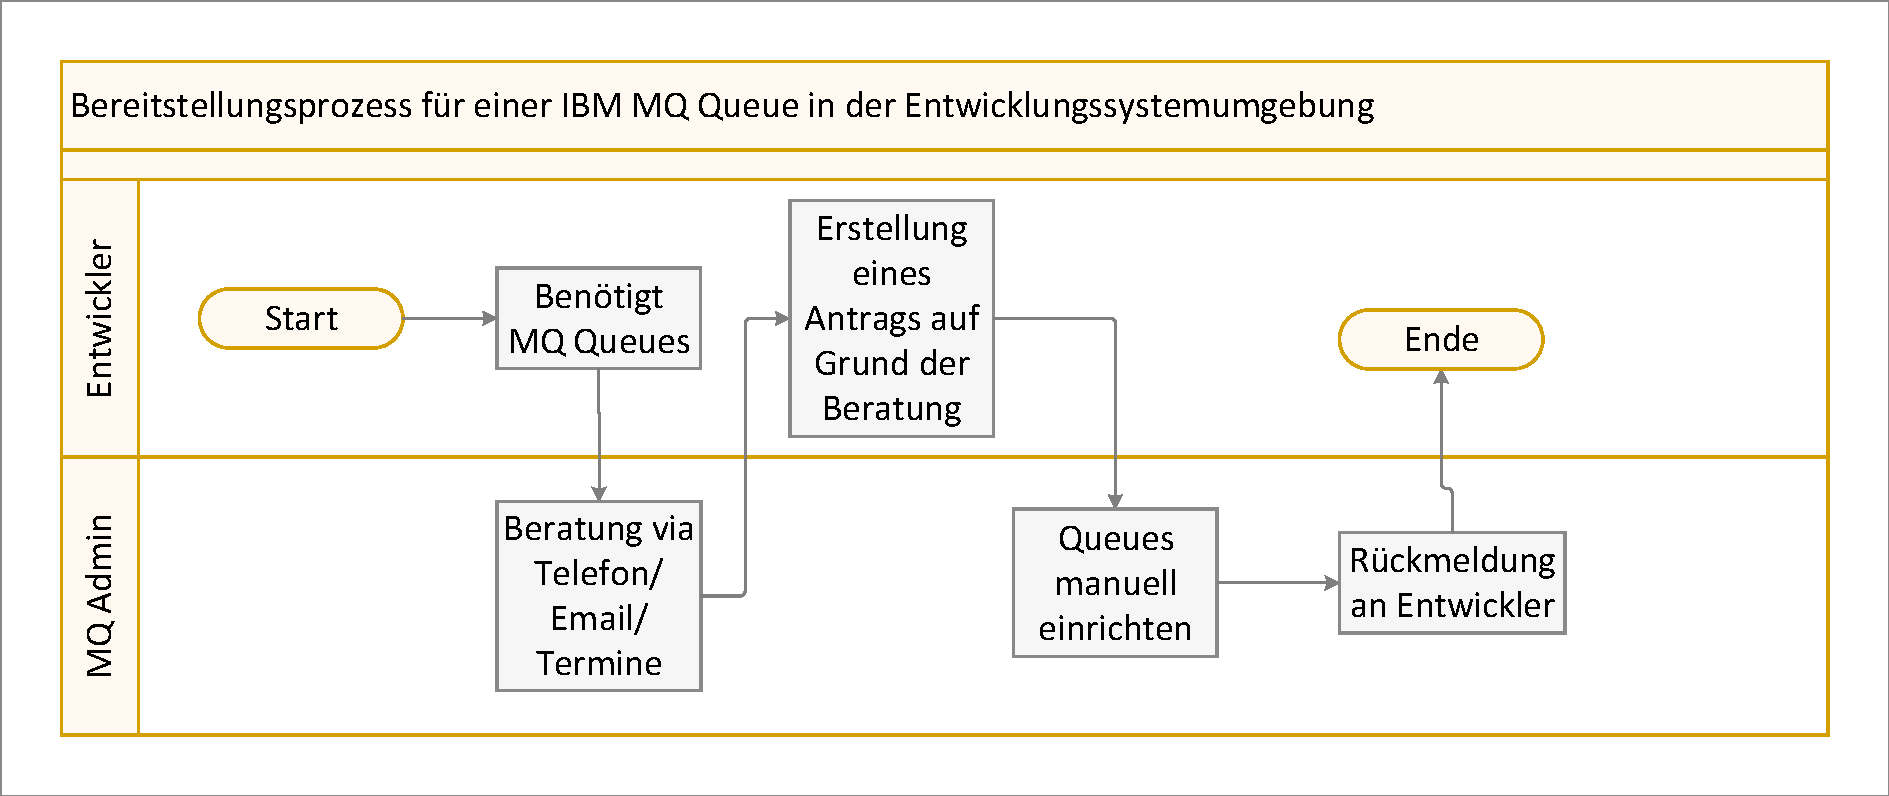
\includegraphics[width=\textwidth]{figures/swimlaneMQ.pdf}
\caption{Bereistellungsprozess von MQ}
\label{fig:aktmq}
\end{figure}
Wie in den drei Diagrammen zu erkennen ist, ist der aktuelle Bereitstellungsprozess noch mit vielen manuellen Schritten verbunden.
Außerdem ist der Hauptaufwand in den Administratorenteams angesiedelt.
Das Entwicklerteam ist der Initiator des Ablaufs.
So kümmert es sich um Formulare und die erste Kontaktaufnahme zum Administratorenteam.
Bei dem Bereitstellungsprozess einer Db2 Datenbank muss es außerdem Projekt Informationen, unter anderem Daten der Voruntersuchung, bereitstellen.
Hinzu komm das Erstellen eines Datenbankmodells.
Hierfür wird Datenbankwissen benötigt. (Kommentar: das wird doch normalerweise in Zusammenarbeit mit der DBA gemacht, oder?

Zusätzlich zu den vielen manuellen Schritten sind die vielen Absprachen zwischen mehreren Abteilungen zu nennen.
Steht ein beteiligtes Team nicht zu Verfügung steht, kommt es zu Verzögerungen, das Team muss warten, der komplette Zeitplan kann sich dadurch nach hinten verschieben.
Der Prozess für die Bereitstellung eines CICS Systems, mit einer Db2 Datenbank und MQ Queues dauert in der Summe circa sechs Arbeitstage.
Es setzt sich aus der Dauer der Einzelnenprozesse zusammen, für jedes Subsystem wird mit circa zwei Arbeitstage gerechnet.
Diese Einschätzung beruht auf der Annahmen, dass zum einen jedes beteiligte Team nur diese Aufgabe zu erledigen hat und zum anderen jeweils ein Tag für die Beratung durch das jeweilige Administratorenteam veranschlagt wird.
Natürlich ist ein parallelisierter Ablauf der einzelnen Teilprozesse möglich, so kann die Gesamtdauer im besten Fall auf circa zwei bis drei Arbeitstage verkürzt werden.

Ein weiterer Punkt ist, dass die Kommunikation beziehungsweise der Initiator für den Start des gesamten Prozesses meist per Zuruf stattfindet.
So existiert für die erste Kontaktaufnahme kein Formular, keine Automation oder ähnliches.
Zur Kommunikation wird auf E-Mail, Telefon oder mittels Terminen zurückgegriffen.


 
